\documentclass{beamer}
\usepackage{graphicx}
\usepackage[outputdir=./target]{minted}
\usepackage[utf8]{inputenc}

\usetheme{Madrid}
\usecolortheme{dolphin}

\graphicspath{ {images/} }

\title{Degasolv}
\subtitle{A Generic Dependency Resolver}
\author{Daniel Jay Haskin}
\begin{document}
\begin{frame}
  \titlepage
\end{frame}
\begin{frame}
  \centerline{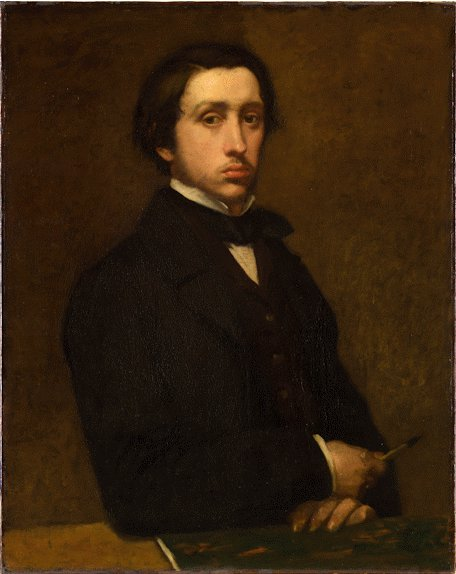
\includegraphics[scale=0.5]{Edgar_Degas_self_portrait_1855.jpeg}}
\end{frame}
\begin{frame}
  \centerline{
\includegraphics[scale=0.15]{DanielHaskin-small.jpg}}
  \center{
    Daniel Jay Haskin \\
    @djhaskin987
  }
\end{frame}
\begin{frame}[fragile]
  \centerline{\color{blue}\Large Dependencies Are The Worst}
\end{frame}
\begin{frame}
    \frametitle{What is Degasolv?}
  \begin{itemize}
      \item Generic dependency tracker with an eye for building and shipping
          software.
      \item Associates something's name, version, and location together
      \item Location can be anything
  \end{itemize}
\end{frame}

\begin{frame}
    \frametitle{Possible Use Cases}
    \begin{itemize}
        \item Track dependencies between build artifacts of different
            languages, new languages, DSLs, C/C++
        \item Download artifacts built by different teams to create a
            product installer
        \item Track dependencies between microservices and use this information
            to determine what services need to be redeployed/restarted
            when a downstream service is changed
    \end{itemize}
\end{frame}
\begin{frame}
  \centerline{
\includegraphics[scale=0.5]{gitsubmodules.jpg}}
\end{frame}
\begin{frame}
  \frametitle{Why Degasolv?}

  Does this sound like problems you deal with?

  \break

  \begin{itemize}
  \item Lots of first party dependencies within the product
  \item All (or lots) of the product's third-party dependencies are built
      on-site
  \item Some languages/technologies don't have a dependency manager
  \item Cross-technology dependencies
  \item Deal with site-specific quirks
  \end{itemize}

  \break

  Then degasolv may be for you.

\end{frame}
\begin{frame}
  \frametitle{Design Goals}
  \begin{itemize}
  \item Degasolv is designed specifically for use by build and DevOps engineers
  \item Degasolv is a ``closed diamond'' resolver
  \item If Degasolv makes you angry, then there is a bug in Degasolv.
  \end{itemize}
  \centerline{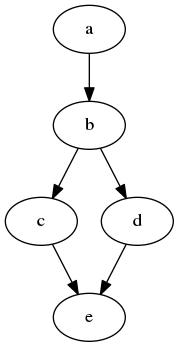
\includegraphics[scale=0.5]{diamonddep.png}}
\end{frame}
\begin{frame}
  \frametitle{Overview}
  \begin{itemize}
  \item Docs: {\small http://degasolv.readthedocs.io/en/latest/}
  \item CLI tool designed for use within a build script
  \item Command-line interface tool
  \item Distributed as a JAR file; runs on the JVM
  \end{itemize}
\end{frame}
\begin{frame}
  \frametitle{Operations}
  \begin{itemize}
      \item \texttt{generate-card}: Generate a \textit{card file} which
          represents a \textit{package}
  \item Upload the card file to a NAS or other central file share
  \item \texttt{generate-repo-index}: Generate a \textit{repository index}
    based on the card files in the central file share
  \item \texttt{resolve-locations}: Using repository indices, find the
      locations of packages and their dependencies
  \item \texttt{query-repo}: Inspect what packages exist in the repository
  \end{itemize}
\end{frame}
\begin{frame}
  \frametitle{What is a Degasolv ``Package''?'}
  \begin{itemize}
  \item A name
  \item A version
  \item A location (URL, file path, bad driving directions...)
  \item A list of dependencies
  \end{itemize}
\end{frame}
\begin{frame}
  \frametitle{Requirement Overview}
  \begin{itemize}
      \item A \textit{requirement} is a predicate describing a package, given
          as a string.
  \item Sort of its own mini language, but it should look familiar
  \item Used in \texttt{generate-card} to specify dependencies
  \item Used in \texttt{resolve-locations} to specify what packages to resolve
  \item Subset of the language used in \texttt{query-repo} to query repository
      for matching packages
\item Specify version ranges and exceptions
  \item Supports boolean operators
  \item Consult the docs for more info
  \end{itemize}
\end{frame}
\begin{frame}[fragile]
  \frametitle{Requirement Examples}
\begin{verbatim}
    "oak"
    "pine>1.0"
    "hickory>1.0,<=2.0"
    "fir<=2.0;>3.5,!=3.8"
    "oak|pine>5.0"
    "hickory>=3.0,<4.0"
    "!birch|birch<=3.0", "!birch>3.0"
    "!oak|maple>3.0"
    "oak|!pine"
\end{verbatim}
\end{frame}
\begin{frame}
  \frametitle{\texttt{generate-card} Overview}
  \begin{itemize}
  \item Generates card files, which contain data about a particular package
  \item Keeps track of dependency information indepently of actual package or
      service
  \item As a convention, it's good to name your card file after the file or
      service to which the its location points (e.g.,
          \texttt{e-1.8.0.zip.dscard}, \texttt{p-dc1-devopsconsul.dscard})
  \item Using card files as in place of actual build artifacts makes
    dependency resolution a completely independent part of your build; you
    don't have to ask developers to change the product to use it.
  \end{itemize}
\end{frame}
\begin{frame}[fragile]
  \frametitle{\texttt{generate-card} Example}
\begin{minted}{bash}
    java \
        -jar ./degasolv-1.0.2-standalone.jar \
        generate-card \
        --id "d" \
        --version "0.8.0" \
        --location "https://example.com/repo/d-0.8.0.zip" \
        --requirement "e>=1.1.0,<2.0.0" \
        --card-file $PWD/d-0.8.0.zip.dscard
\end{minted}
\end{frame}
\begin{frame}[fragile]
  \frametitle{\texttt{generate-card} Output: The \texttt{*.dscard} File}
\begin{minted}[fontsize=\footnotesize]{clojure}
    ; Filename: d-0.8.0.dscard
    #degasolv.resolver/PackageInfo {
        :id "d",
        :version "0.8.0",
        :location "https://example.com/repo/d-0.8.0.zip",
        :requirements [ [
            #degasolv.resolver/Requirement {
                :status :present,
                :id "e",
                :spec [ [
                    #degasolv.resolver/VersionPredicate {
                        :relation :greater-equal,
                        :version "1.1.0"}
                    #degasolv.resolver/VersionPredicate {
                        :relation :less-than,
                        :version "2.0.0"
                    }
                ]]
            }
        ]]
    }
\end{minted}
\end{frame}
\begin{frame}[fragile]
  \frametitle{\texttt{generate-card} Final Step: Deposit the Card File}
  \begin{itemize}
  \item After the card file is generated, it needs to be deposited into a
    central file share
  \end{itemize}
\begin{minted}{bash}
    $ find .
    .
    ./c-3.5.0.zip.dscard
    ./b-2.3.0.zip.dscard
    ./e-2.1.0.zip.dscard
    ./e-2.4.0.zip.dscard
    ./e-1.8.0.zip.dscard
    ./d-0.8.0.zip.dscard
    ./c-2.4.7.zip.dscard
\end{minted}
\end{frame}
\begin{frame}
  \centerline{\color{blue}\Large \texttt{generate-card} Demo}
\end{frame}
\begin{frame}
  \frametitle{\texttt{generate-repo-index} Overview}
  \begin{itemize}
  \item Patterned after YUM's \texttt{createrepo}
  \item Running \texttt{generate-repo-index} from the directory containing \texttt{*.dscard}
    files
  \item The index will then contain information about packages represented in those
    files
  \end{itemize}
\end{frame}
\begin{frame}[fragile]
  \frametitle{\texttt{generate-repo-index} Example}
  Command:
\begin{minted}[fontsize=\footnotesize]{bash}
    java \
        -jar ./degasolv-1.0.2-standalone.jar \
        generate-repo-index \
        --search-directory $PWD \
        --index-file $PWD/index.dsrepo
\end{minted}
  Result:
\begin{minted}[fontsize=\footnotesize]{bash}
    $ find .
    .
    ./c-3.5.0.zip.dscard
    ./b-2.3.0.zip.dscard
    ./e-2.1.0.zip.dscard
    ./e-2.4.0.zip.dscard
    ./e-1.8.0.zip.dscard
    ./d-0.8.0.zip.dscard
    ./c-2.4.7.zip.dscard
    ./index.dsrepo # <----- new file
\end{minted}
\end{frame}
\begin{frame}
  \centerline{\color{blue}\Large \texttt{generate-repo-index} Demo}
\end{frame}
\begin{frame}
  \frametitle{\texttt{resolve-locations} Overview}
  \begin{itemize}
  \item This command resolves dependencies given a target expression
  \item The names, versions, and locations of the resolved packages are printed
  \item The output is designed to be both machine and human readable
  \item Command is designed to be used within build scripts
  \end{itemize}
\end{frame}
\begin{frame}[fragile]
  \frametitle{\texttt{resolve-locations} Example}
  Command:
\begin{minted}{bash}
    java \
        -jar ./degasolv-1.0.2-standalone.jar \
        resolve-locations \
        --repository $PWD/index.dsrepo \
        --requirement "b"
\end{minted}
  Output:
\begin{verbatim}
    c==3.5.0 @ https://example.com/repo/c-3.5.0.zip
    d==0.8.0 @ https://example.com/repo/d-0.8.0.zip
    e==1.8.0 @ https://example.com/repo/e-1.8.0.zip
    b==2.3.0 @ https://example.com/repo/b-2.3.0.zip
\end{verbatim}
\end{frame}
\begin{frame}
  \centerline{\color{blue}\Large \texttt{resolve-locations} Demo}
\end{frame}

\begin{frame}
  \frametitle{\texttt{query-repo} Overview}
  \begin{itemize}
  \item This command allows the user to query the repository index directly
  \item Implemented to allow engineers to debug builds
  \end{itemize}
\end{frame}
\begin{frame}[fragile]
  \frametitle{\texttt{query-repo} Example}
  Command:
\begin{minted}{bash}
    java \
        -jar ./degasolv-1.0.2-standalone.jar \
        --config-file $PWD/config.edn \
        query-repo \
        --query "e>2.0.0,!=2.1.0"
\end{minted}
  Output:
\begin{verbatim}
    e==2.4.0 @ https://example.com/repo/e-2.4.0.zip
\end{verbatim}
\end{frame}

\begin{frame}
  \centerline{\color{blue}\Large \texttt{query-repo} Demo}
\end{frame}
\begin{frame}
  % For this demo we will do multi-technology and native in the same demo,
  % Patterned after what I've seen before, but also patterned after the
  % 'Longer Example' I gave in the docs.
  \centerline{\color{blue}\Large Demo}
\end{frame}
\begin{frame}[fragile]
  \frametitle{JFrog Artifactory Integration}
  \begin{itemize}
  \item JFrog artifactory CLI already pairs well with degasolv
  \end{itemize}
\end{frame}
\begin{frame}[fragile]
\frametitle{JFrog Artifactory Integration: Setup}
\begin{minted}[fontsize=\footnotesize]{bash}
    #!/bin/sh

    package_name="top"
    build_name="jenkins-${package_name}"
    build_number="18"

    jfrog rt build-clean "${build_name}" "${build_number}"
    jfrog rt build-collect-env "${build_name}" "${build_number}"
    jfrog rt build-add-git "${build_name}" "${build_number}"
\end{minted}
\end{frame}
\begin{frame}[fragile]
\frametitle{JFrog Artifactory Integration: Download}
\begin{minted}[fontsize=\footnotesize]{bash}
    mkdir -p deps
    for loc in $(java \
        -jar ./degasolv-1.0.2-standalone.jar \
        resolve-locations \
        --repository=<ARTIFACTORY-REPO-URL>/index.dsrepo \
        top_dep_a top_dep_b top_dep_c | \
        awk -F' *@ *' '{print $2}')
    do
        # The `loc` var holds a location of the form
        # `<artifactory-repo>/<path-to-artifact>`
        jfrog rt download \
            --build-name "${build_name}" \
            --build-number "${build_number}" \
            "${loc}"
            ./deps
    done
\end{minted}
\end{frame}
\begin{frame}[fragile]
\frametitle{JFrog Artifactory Integration: Upload}
\begin{minted}[fontsize=\footnotesize]{bash}
    jfrog rt upload \
        --build-name "${build_name}" \
        --build-number "${build_number}" \
        ./target/<artifact> \
        <artifactory-repo>/<path-to-artifact>
    jfrog rt upload \
        --build-name "${build_name}" \
        --build-number "${build_number}" \
        ./target/<artifact>.dscard \
        <artifactory-degasolv-repo>/<path-to-card>.dscard
    jfrog rt build-publish "${build_name}" "${build_number}"
\end{minted}
\end{frame}
\begin{frame}[fragile]
\frametitle{JFrog Artifactory Integration: Index}
\begin{minted}[fontsize=\footnotesize]{bash}
    java \
        -jar ./degasolv-1.0.2-standalone.jar \
        generate-repo-index \
        --search-directory $PWD \
        --add-to <artifactory-degasolv-repo>/<path-to-index>.dsrepo \
        --index-file $PWD/index.dsrepo
    curl -i -H 'X-JFrog-Art-Api: <API-KEY>' \
        -XPOST \
        <artifactory-degasolv-repo>/<path-to-index>.dsrepo \
        -T $PWD/index.dsrepo
\end{minted}
\end{frame}
\begin{frame}
  \frametitle{JFrog Artifactory Integration: Result}
  \begin{itemize}
  \item Degasolv resolves the dependencies for this particular artifact
  \item Artifacts that were downloaded via \texttt{jfrog rt download} are listed as
    dependencies to the build artifacts
  \item Build information for your artifact is published
  \item Artifacts were uploaded via \texttt{jfrog rt upload}
  \item Repository index is updated*
  \end{itemize}
\end{frame}
\begin{frame}
  \frametitle{Summary}
  \begin{itemize}
  \item Degasolv helps you manage out-of-control first party and third party dependencies
  \item Degasolv can be implemented without asking developers to change the contents
    of build artifacts
  \item Degasolv is specifically designed for build engineers who are responsible for
    many different types of builds
  \item Degasolv integrates cleanly into existing build scripts and infrastructure (e.g.
    Artifactory or a build artifact NAS)
  \end{itemize}
  \end{frame}
\begin{frame}
  \frametitle{Community}
  \textit{To use a thing, join its people.}

  \break

  \begin{itemize}
  \item Gitter room ``degasolv'' \\
    {\small https://gitter.im/degasolv/Lobby}
  \item Google group ``degasolv-users'' \\
    {\small https://groups.google.com/forum/\#!forum/degasolv-users}
  \end{itemize}
\end{frame}
\begin{frame}
  \frametitle{Future Directions}
  \begin{itemize}
  \item JFrog Artifactory plugin
  \item Resolution directly from different types of repositories
  \item Homebrew \\
    {\small https://github.com/Homebrew/brew/blob/master/docs/Formula-Cookbook.md}
  \item RPM, Debian packages
  \end{itemize}
\end{frame}
\begin{frame}
  \frametitle{Further Reading}
  \begin{itemize}
  \item Kill Your Dependencies {\small http://www.mikeperham.com/2016/02/09/kill-your-dependencies/}
  \item Embracing Conway's Law {\small https://wingolog.org/archives/2015/11/09/embracing-conways-law}
  \item JFrog Artifactory CLI {\small https://www.jfrog.com/confluence/display/CLI/CLI+for+JFrog+Artifactory}
  \item So You Want to Write a Package Manager {\small https://yarnpkg.com/blog/2016/11/24/lockfiles-for-all/}
  \item Lockfiles should be committed on all projects {\small https://yarnpkg.com/blog/2016/11/24/lockfiles-for-all/}
  \end{itemize}
\end{frame}
\begin{frame}
  \centerline{\color{blue}\Large Questions}
\end{frame}
\end{document}
